\documentclass[12pt]{exam}
%\documentclass[12pt]{article}
\usepackage[letterpaper, margin=0.75in]{geometry}
\usepackage{graphicx}
\usepackage{enumitem}
\usepackage{booktabs}
\usepackage{amsmath}
\usepackage{tabularx}
\usepackage{color}
\usepackage{textcomp}

\begin{document}
\footer{}{Page \thepage\ of \numpages}{}

\begin{center}

\includegraphics[width=10cm]{../images/logo.png}
\end{center}

\begin{center}
\noindent{\LARGE Conceptual Physics \\ Class 7 Questions \\ March 23, 2018 \\ ~ \\ Practice Questions for First Partial Test \\ SOLUTIONS \\}
\end{center}
\vspace{0.2in}

\clearpage
\begin{questions}

\question What is an ideology? What are scientific theories?
	\begin{TheSolution}
	An ideology is a set of ideas. Scientific theories are the set of \textit{falsifiable} (can be proven wrong) ideas that have withstood extensive scrutiny and experimental testing. They contain explanatory and predictive power: They can predict the outcome of an experiment or test.
	\end{TheSolution}
	
\question
Some philosophers assert that there is no difference between science and myth, and that modern science fills the same role as ancient myth, with no difference in its methods. What do you think? In what ways are modern science and ancient mythology similar and/or different?
\begin{TheSolution}
Like myths, science attempts to create a coherent worldview---to answer questions about why the world is the way it is and how we got here. Like myth, belief in the value of science causes people to perform ritualistic behaviors (\textit{e.g.}, performing research), but it is not always clear why we need to perform these rituals, since their benefits cannot always be demonstrated. The benefits of science are often described to the general public using the same terms as ancient myths: the promise of allowing us to control nature and become perfect and god-like (\textit{e.g.}, the promises of modern medicine being similar to mythological promises of immortality and eternal youth). These philosophers see scientists as using their position of authority to convince the general public of the truth of their claims, rather than using a thorough explanation of the scientific process, so to them, a lay person's belief in science is the same as their ancestors' belief in the myths their shamans told them. Moreover, they see scientists as clinging dogmatically to a worldview which cannot completely describe reality but that they refuse to admit is incomplete, the way ancient humans clung to myths that were internally inconsistent.

This last claim is the most confusing; the whole point of science is to try to \textit{improve} our understanding of the physical world, which is not consistent with a belief that our current understanding of the physical world is complete. A physicist who believed that our current physical theories perfectly describe reality would not be a very good physicist, since there would be nothing left for them to do.
While the results of modern science might be of mixed or questionable benefit to society (antibiotics, anesthetics, and vaccines \textit{vs.} climate change), they have nevertheless been \textit{different} to the results of a mythological understanding of the world. For example, for thousands of years humans have been trying to understand the motion of objects in the sky and how those objects got there but made almost no progress until the last few hundred years. Given that those early humans' brains were almost the same as ours, it is hard to explain why they failed and we succeeded without accepting that the way modern scientists seek explanations (through gathering data and rigorously testing ideas) and the kind of explanations they seek (theories with predictive and explanatory power) are fundamentally different from a mythological approach. As long as you accept that there is some physical reality external to your mind and that it is possible for us to gain information about that reality, it is hard to dispute that modern science does a better job of giving us information about reality than ancient myth. It seems questionable to suggest that a belief that the Sun is pulled across the sky every day by a god in a chariot is equivalent to a belief that the Earth and the Moon follow orbits described by Newtonian gravity when one of those beliefs allows you to accurately predict eclipses years in advance and the other cannot even assure you that the Sun will rise tomorrow.
\end{TheSolution}

\question
	Convert the following to centimeters (cm). Some useful conversion factors: 1~mile = 1.6~km, 1~light-year = $9\times 10^{15}~m$.
	
		\begin{parts}
		\part 15~m
			\begin{TheSolution}
				\begin{eqnarray}
				15~m\times\frac{100~cm}{1~m} = 1500~cm \nonumber
				\end{eqnarray}
			\end{TheSolution}
		\part 10~miles
			\begin{TheSolution}
				\begin{eqnarray}					
				10~miles \times\frac{1.6~km}{1~mile} \times \frac{10^3~m}{1~km} \times \frac{10^2~cm}{1~m } = 1.6 \times 10^6~cm \nonumber
				\end{eqnarray}			
			\end{TheSolution}
		\part 2~light-years
			\begin{TheSolution}
				\begin{eqnarray}
				2~lightyears\times \frac{9\times 10^{15}~m}{1~lightyear} \times \frac{10^2~cm}{1~m} = 18\times 10^{17}~cm = 1.8\times 10^{18}~cm\nonumber
				\end{eqnarray}
			\end{TheSolution}
	\end{parts}

\question
You are an astronaut on Mars, passing the time by juggling. You are taking advantage of the fact that the acceleration due to gravity on the surface of Mars is only about 4 m/s$^2$, which allows you to have slower reaction times. You throw a ball straight upwards at 8 m/s.
\begin{parts}
\part Draw a sketch of the problem.
\begin{TheSolution}
Here I defined the moment the ball left your hand as $t=0$~s.
\begin{center}
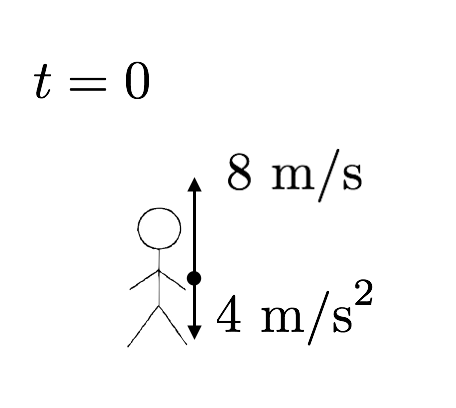
\includegraphics[width=0.4\textwidth]{../images/practice_mars.png}
\end{center}
\end{TheSolution}
\part How long does the ball take to reach the top of its trajectory?
\begin{TheSolution}
The ball reaches the top of its trajectory when it stops going upwards and starts going downwards (when $v=0$). This happens when
\begin{eqnarray}
\Delta t = \frac{8~\text{m/s}}{4~\text{m/s}^2} = 2~\text{s}\nonumber
\end{eqnarray}
\end{TheSolution}
\part How high does the ball go?
\begin{TheSolution}
We know the initial velocity (8 m/s up), acceleration ($4 m/s^2$ down) and the time it takes to travel (2~s). We can therefore use the following equation:
\begin{eqnarray}
x &=& v_0t + \frac{1}{2}at^2 \nonumber \\
&=& 8 m/s \times 2 s + \frac{1}{2} (-4 m/s^2) \times (2 s)^2 \nonumber \\
&=& 16 m - 8 m \nonumber \\
&=& 8 m \nonumber
\end{eqnarray}
Another way to view this problem is that, because the ball is undergoing constant acceleration, the ball's average velocity during this interval is just the average of its initial and final velocity,
\begin{eqnarray}
\bar{v} = \frac{8~\text{m/s}+0~\text{m/s}}{2} = 4~\text{m/s}\nonumber
\end{eqnarray}
At this average velocity over an interval of 2 s, it travels
\begin{eqnarray}
\Delta x = 4~\text{m/s}\times 2~\text{s} = 8~\text{m}\nonumber
\end{eqnarray}
\end{TheSolution}
\part How long does the ball take to land back in your hand, from the moment you threw it?
\begin{TheSolution}
On the way back to its initial height, the ball's trajectory is the exact reverse, and it takes the same length of time (2 s) so the total length of time from when you threw it to when you caught it is 4 s.
\end{TheSolution}
\end{parts}


\question
The following velocity \textit{vs.} time plot describes the random motion of someone running back and forth on a sidewalk. Let the positive direction indicate East, and negative direction be West.

\begin{center}
\noindent 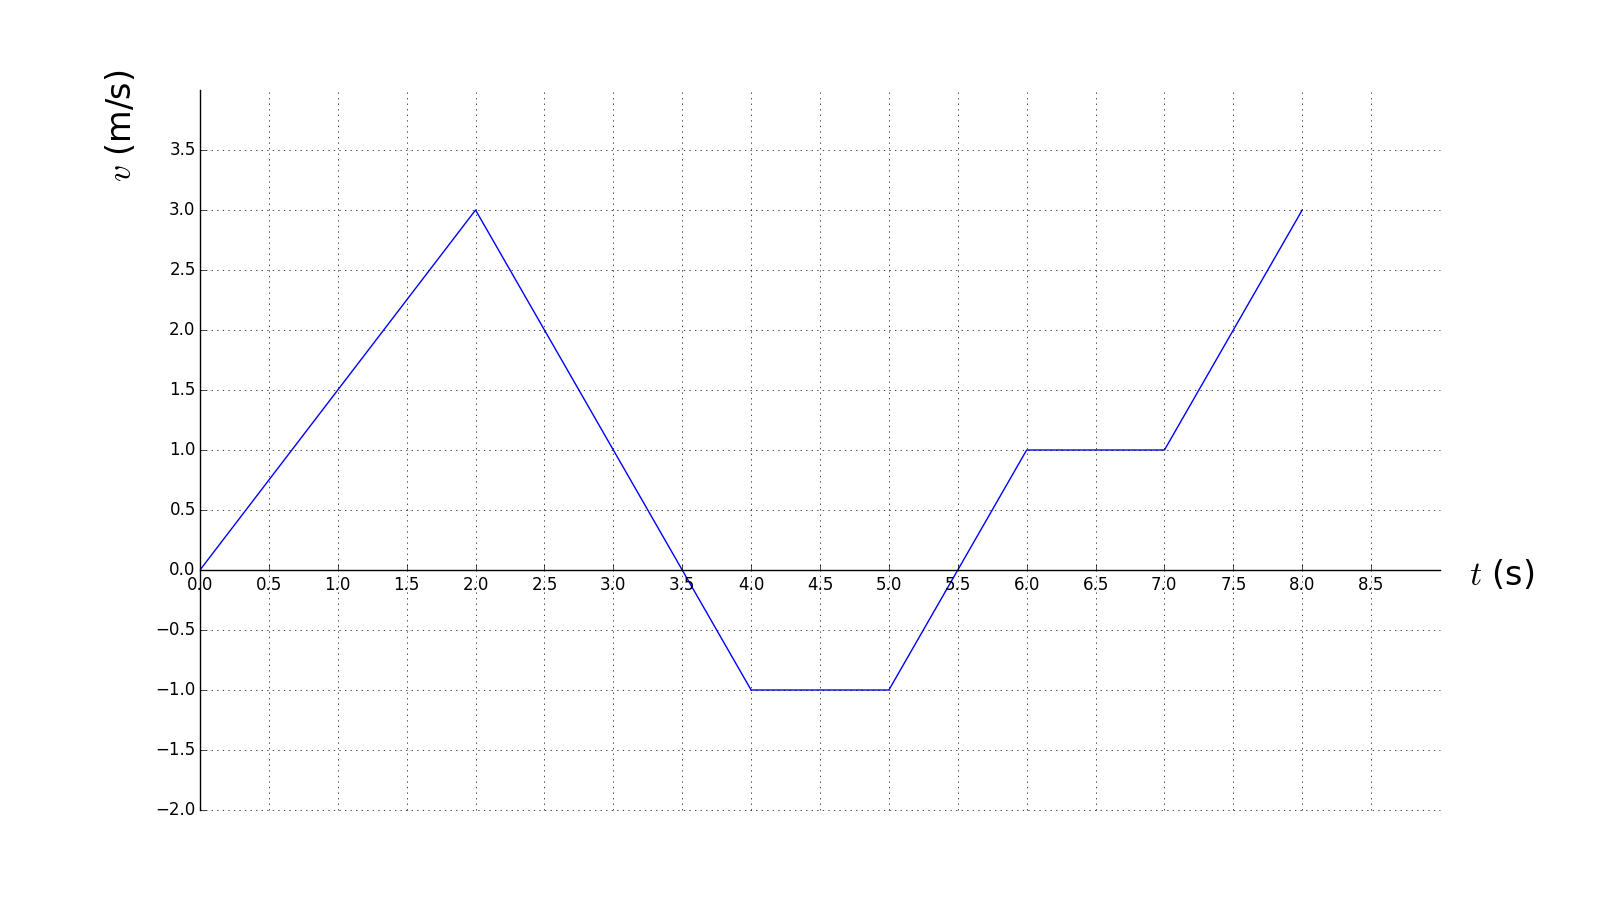
\includegraphics[width=0.9\textwidth]{../images/practtest1_plot.png}
\end{center}

\begin{parts}
\part When were they moving fastest?
\begin{TheSolution}
At t=2 s, and again at t=8 s.
\end{TheSolution}
\part What was their greatest velocity?
\begin{TheSolution}
3 m/s
\end{TheSolution}
\part When were they not moving?
\begin{TheSolution}
They were not moving when the velocity = 0, which happened at t=0 s, t=3.5 s, t=5.5 s
\end{TheSolution}
\part When was their acceleration zero?
\begin{TheSolution}
A zero acceleration means velocity isn't changing. This happens when the velocity vs. time graph is flat: between t=4 s and t=5 s, and again between t = 6 s and t=7s.
\end{TheSolution}
\part When was their acceleration negative?
\begin{TheSolution}
When the velocity vs. time graph slopes down, acceleration is negative. This happens between t=2 s and t=4 s.
\end{TheSolution}
\end{parts}

\question
Despite a very strong wind, a tennis player manages to hit a tennis ball with her racquet so that the ball passes over the net and lands in her opponent's court. Consider the following forces:
\begin{enumerate}
\item A downward force of gravity
\item A force by the ``hit''
\item A force exerted by the air
\end{enumerate}
Which of the above forces is (are) acting on the tennis ball after it has left contact with the racquet and before it touches the ground?
\begin{choices}
\choice 1 only
\choice 1 and 2
\choice 1 and 3
\choice 2 and 3
\choice 1, 2, and 3
\end{choices}
\begin{TheSolution}
\textbf{C}. The ball has left contact with the racquet so it no longer experiences a force from the hit; the only forces acting on it are gravity and the wind (the problem says there is a very strong wind so you know not to ignore air resistance in this problem).
\end{TheSolution}

\question
The figure depicts a hockey puck sliding with a constant speed $v_0$ from point $a$ to point $b$ on a frictionless horizontal surface. Forces exerted by the air are negligible. You are looking down on the puck. When the puck reaches point $b$, it receives a swift horizontal kick in the direction of the heavy print arrow.
\begin{center}
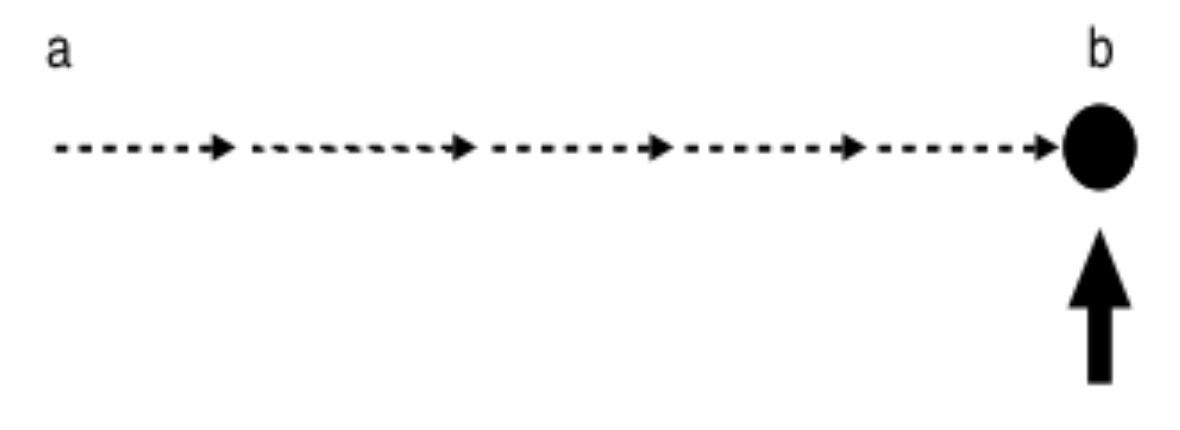
\includegraphics[width=0.8\textwidth]{../images/FCI_puck1.png}
\end{center}
\begin{parts}
\part
Which of the paths below would the puck most closely follow after receiving the kick?

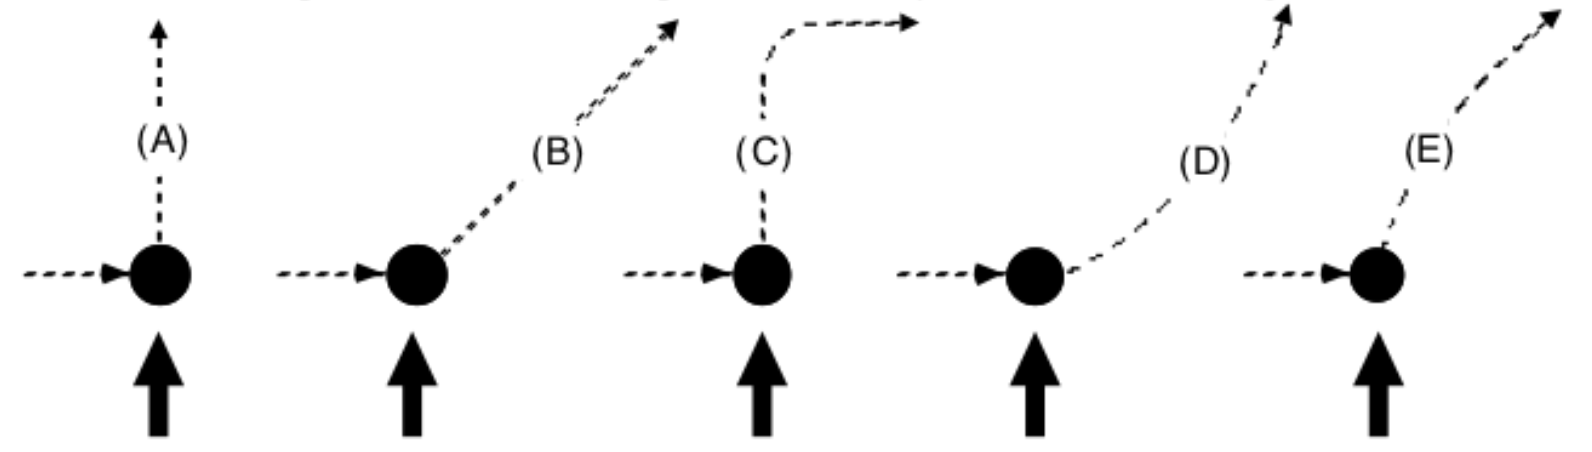
\includegraphics[width=0.8\textwidth]{../images/FCI_puck2.png}
\begin{TheSolution}
\textbf{B}. The problem says the puck receives a \textit{swift} kick so we know the interval over which the force was acting on the puck was very brief; we can treat it as an infinitesimal impulse, adding a constant northward component to the puck's velocity. This does not change the puck's eastward motion, which also remains constant, so the puck moves diagonally in a straight line at a constant velocity after the kick.
\end{TheSolution}

\part
Along the frictionless path you have chosen above, the speed of the puck after receiving the kick:
\begin{choices}
\choice is constant.
\choice continuously increases.
\choice continuously decreases.
\choice increases for a while and decreases thereafter.
\choice is constant for a while and decreases thereafter.
\end{choices}
\begin{TheSolution}
\textbf{A}. As stated above.
\end{TheSolution}

\part
Along the frictionless path you have chosen above, the main force(s) acting on the puck after receiving the kick is (are):
\begin{choices}
\choice a downward force of gravity.
\choice a downward force of gravity, and a horizontal force in the direction of motion.
\choice a downward force of gravity, an upward force exerted by the surface, and a horizontal force in the direction of motion.
\choice a downward force of gravity and an upward force exerted by the surface.
\choice none. (No forces act on the puck.)
\end{choices}
\begin{TheSolution}
\textbf{D}. If it were only the force of gravity, the puck would accelerate down. An upward contact force from the surface is needed to ensure that the net force acting on the puck is zero (which is why it isn't accelerating)
\end{TheSolution}
\end{parts}

\question
You are hiking on a glacier and come across a crevasse. It is too narrow for you to see the bottom, but you want to know how deep it is, so you drop a rock straight down ($v_0 = 0$~m/s) and listen for a splash, which you hear 2.0 s later. (For simplicity, assume the acceleration due to gravity is 10 m/s$^2$ downwards.)
\begin{parts}
\part Draw a sketch of the problem.
\begin{TheSolution}
\begin{center}
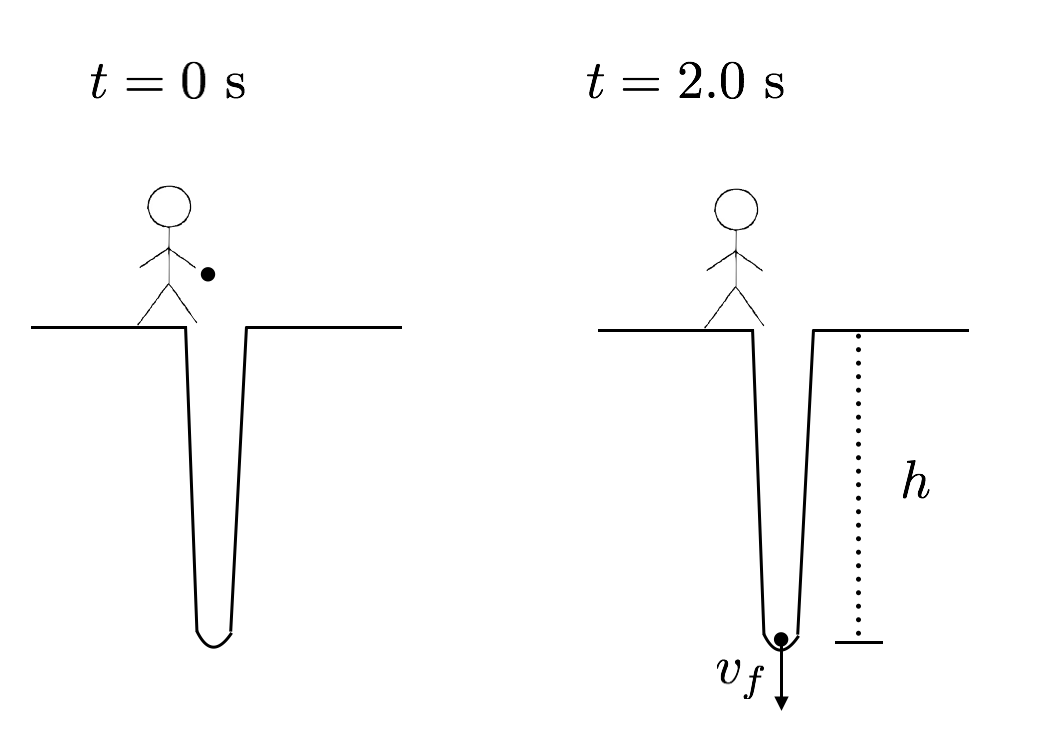
\includegraphics[width=\textwidth]{../images/test1_glacier.png}
\end{center}
\end{TheSolution}
\part What was the rock's velocity when it hit the bottom?
\begin{TheSolution}
The rock accelerates 10 meters per second per second, so in 2 seconds it accelerates to 20 m/s (-20 m/s if you define downwards as negative).
\end{TheSolution}
\part What was the rock's average velocity during the fall?
\begin{TheSolution}
Since the rock is undergoing constant acceleration, its average velocity is the average of the initial and final velocities,
\begin{eqnarray}
\bar{v} = \frac{v_0 + v_f}{2} = \frac{0~\text{m/s} -20~\text{m/s}}{2} = -10~\text{m/s} \nonumber
\end{eqnarray}

\end{TheSolution}
\part How deep is the crevasse?
\begin{TheSolution}
There are two possible ways to solve this problem.

(1) The rock's displacement is its average velocity times the elapsed time, $-10~\text{m/s}\cdot 2~\text{s}=-20~\text{m}$---that is, the rock drops 20 m; the crevasse is 20 m deep.

(2) Alternatively, we know the acceleration, time, and initial velocity. We can therefore use:
\begin{eqnarray}
x &=& v_0 t + \frac{1}{2} a t^2 \nonumber \\
&=& \frac{1}{2}(10~m/s^2) (2s)^2 \nonumber \\
&=& 20~m \nonumber
\end{eqnarray}
\end{TheSolution}
\end{parts}

\question
The following position \textit{vs.} time plot describes the motion of a toy train being pushed along a straight track, where $x=0$ is the center of the track and points to the right are positive. For questions that ask you to list points, \textbf{refer only to the labeled points.}

\begin{center}
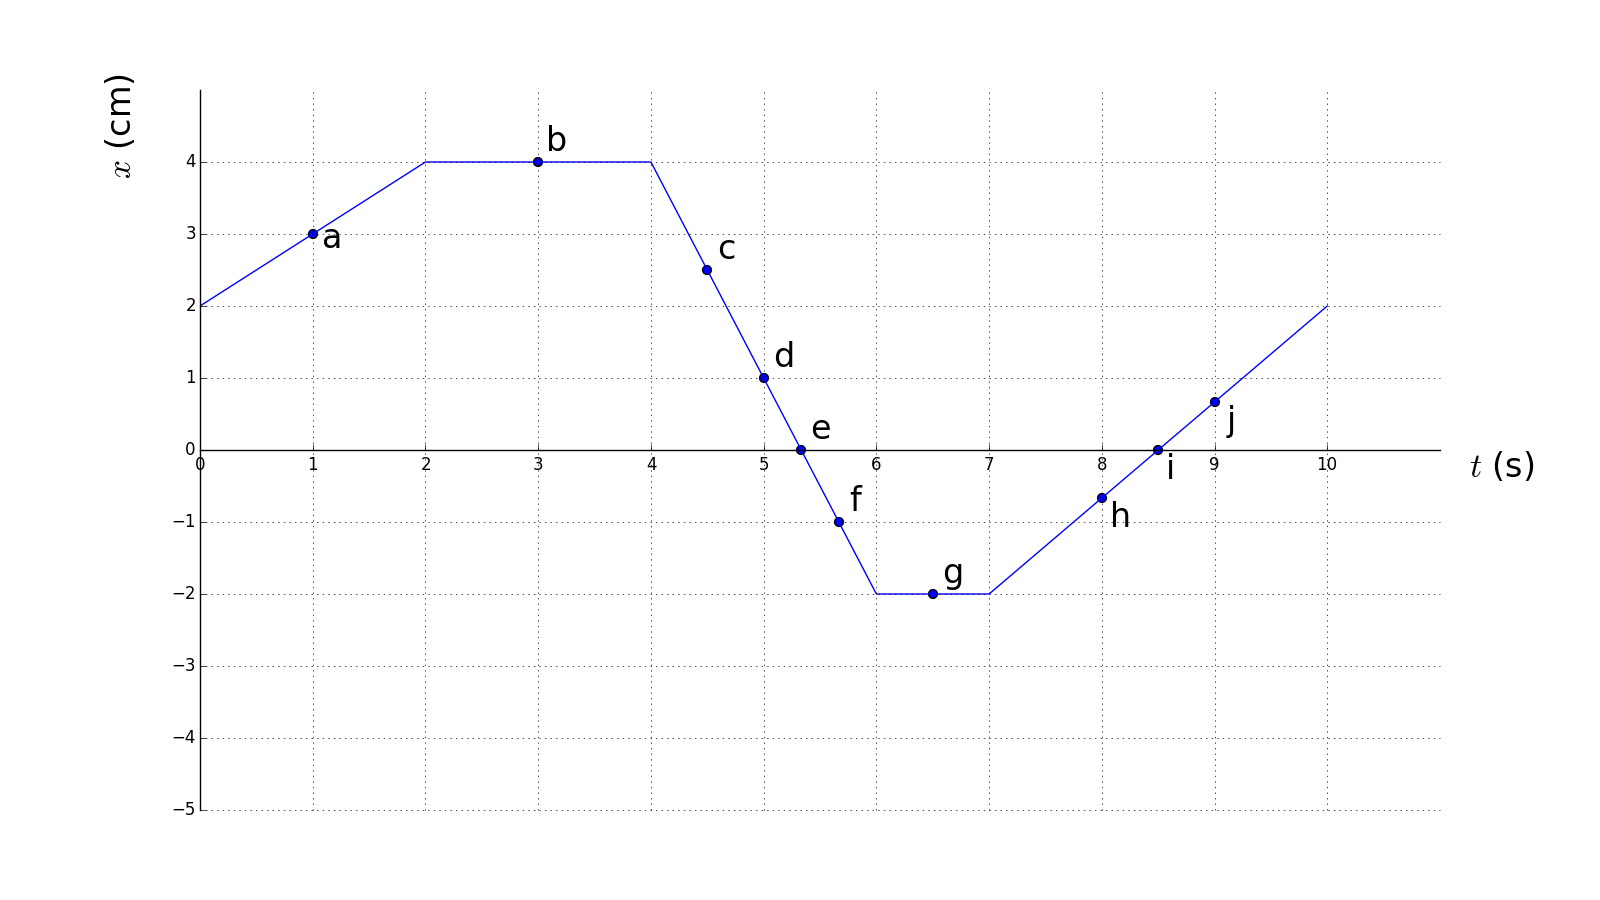
\includegraphics[width=\textwidth]{../images/test1_plot.png}
\end{center}

\begin{parts}
\part At which point(s) is the train not moving?
\begin{TheSolution}
\textbf{b, g}: The train is not moving when position is constant (when the slope is zero).
\end{TheSolution}
\part At which point(s) is the train moving fastest?
\begin{TheSolution}
\textbf{c, d, e, f}: The train is moving the fastest when the magnitude of its velocity is greatest; since velocity is the slope of a position \textit{vs.} time plot, this is when the slope is steepest.
\end{TheSolution}
\part At which point(s) is the train farthest to the left?
\begin{TheSolution}
\textbf{g}: This is when $x$ is the most negative.
\end{TheSolution}
\part At which point(s) is the train \textit{moving} to the left?
\begin{TheSolution}
\textbf{c, d, e, f}: The train is moving left whenever its velocity is negative; in other words, whenever the slope is negative.
\end{TheSolution}
\part At which point(s) does the train experience zero acceleration?
\begin{TheSolution}
\textbf{a, b, c, d, e, f, g, h, i, j}: At every labeled point on this graph, slope is constant (they are all straight line segments), meaning velocity is constant, meaning there is zero acceleration.
\end{TheSolution}
\part What is the train's displacement from $t=0$ to $t=10$~s?
\begin{TheSolution}
It starts and ends at $x=2$ cm, so its displacement is 0 cm.
\end{TheSolution}
\end{parts}

\question
A boy throws a steel ball straight up. Consider the motion of the ball only after it has left the boy's hand but before it touches the ground, and assume that forces exerted by the air are negligible. For these conditions, the force(s) acting on the ball is (are):
\begin{choices}
\choice a downward force of gravity along with a steadily decreasing upward force.
\choice a steadily decreasing upward force from the moment it leaves the boy's hand until it reaches its highest point; on the way down there is a steadily increasing downward force of gravity as the object gets closer to the earth.
\choice an almost constant downward force of gravity along with an upward force that steadily decreases until the ball reaches its highest point; on the way down there is only a constant downward force of gravity.
\choice an almost constant downward force of gravity only.
\choice none of the above. The ball falls back to the ground because of its natural tendency to rest on the surface of the earth.
\end{choices}
\begin{TheSolution}
\textbf{D}. The problem says to consider the motion of the ball \textit{after it has left the boy's hand but before it touches the ground}; nothing is pushing up on it during this time.
\end{TheSolution}
\question
\label{ques:25}
A woman exerts a constant horizontal force on a large box. As a result, the box moves across a horizontal floor at a constant speed $v_0$.

The constant horizontal force applied by the woman:
\begin{choices}
\choice has the same magnitude as the weight of the box.
\choice is greater than the weight of the box.
\choice has the same magnitude as the total force which resists the motion of the box.
\choice is greater than the total force which resists the motion of the box.
\choice is greater than either the weight of the box or the total force which resists its motion.
\end{choices}
\begin{TheSolution}
\textbf{C}. Since the box is moving at a constant velocity, the net force on it must be zero, so the horizontal force applied by the woman must be canceled out by the force(s) which resist the motion of the box.

\begin{center}
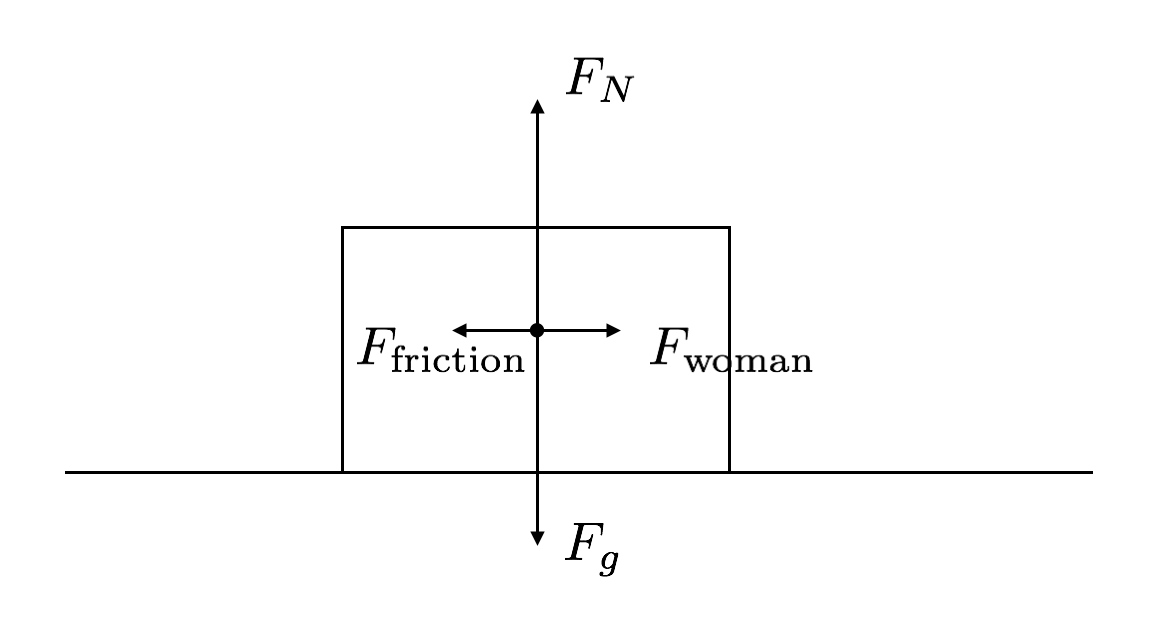
\includegraphics[width=0.8\textwidth]{../images/test1_box1.png}
\end{center}
\end{TheSolution}

\question
If the woman in the previous question doubles the constant horizontal force that she exerts on the box to push it on the same horizontal floor, the box then moves:
\begin{choices}
\choice with a constant speed that is double the speed $v_0$ in the previous question.
\choice with a constant speed that is greater than the speed $v_0$ in the previous question, but not necessarily twice as great.
\choice for a while with a speed that is constant and greater than the speed $v_0$ in the previous question, then with a speed that increases thereafter.
\choice for a while with an increasing speed, then with a constant speed thereafter.
\choice with a continuously increasing speed.
\end{choices}
\begin{TheSolution}
\textbf{E}. The forces are now the ones shown below; the constant horizontal force is no longer canceled by the frictional force, and the box accelerates (to the right in this diagram).

\begin{center}
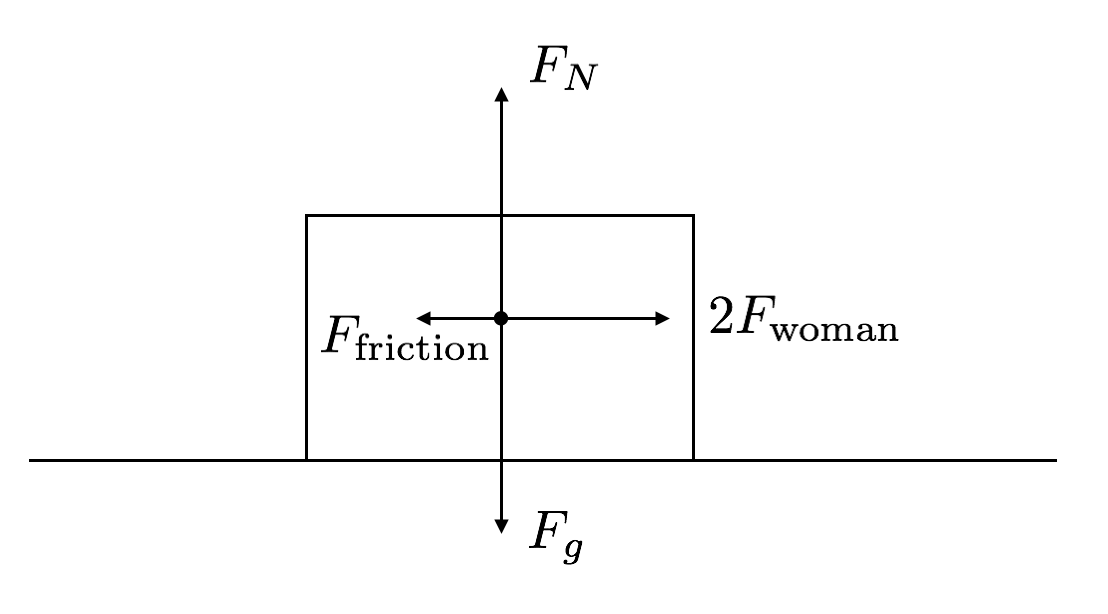
\includegraphics[width=0.8\textwidth]{../images/test1_box2.png}
\end{center}
\end{TheSolution}

\question
If the woman in question~\ref{ques:25} suddenly stops applying a horizontal force to the box, then the box will:
\begin{choices}
\choice immediately come to a stop.
\choice continue moving at a constant speed for a while and then slow to a stop.
\choice immediately start slowing to a stop.
\choice continue at a constant speed.
\choice increase its speed for a while and then start slowing to a stop.
\end{choices}
\begin{TheSolution}
\textbf{C}. The forces are now as shown below. There is no longer a horizontal force to cancel out friction, so there is a net force in the direction opposite to the box's motion, and thus an acceleration opposite to the box's motion, causing it to slow to a stop.

\begin{center}
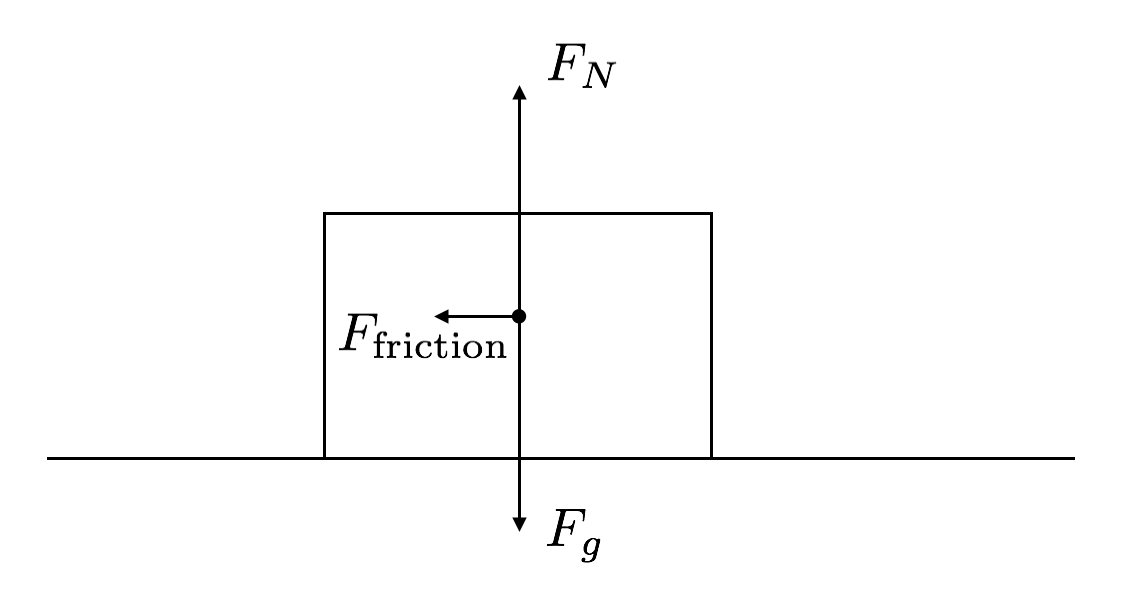
\includegraphics[width=0.8\textwidth]{../images/test1_box3.png}
\end{center}
\end{TheSolution}

\question Consider 2 planets, planet $A$ and planet $B$, orbiting a distant star. The following 3 scenarios have the two planets located at different distances and with varying masses, and will ask you to compare the gravitational forces experienced by them.
\begin{parts}
	\part Planet $A$ and planet $B$ are identical, and orbit the star at different distances. Planet $A$ is \textbf{twice as far away} from the star as planet $B$. Which, if any, experiences the greater gravitational attraction to the star? Why?
	\begin{center}
	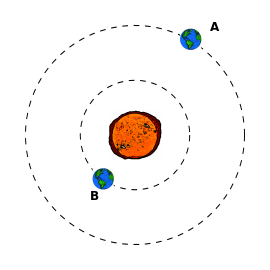
\includegraphics{../images/2PlanetsA.png}
	\end{center}
	
	\begin{TheSolution}
		B. The force of gravity increases as objects are brought closer together. Planet $B$ is closer to the star than planet $A$, so it experiences a greater gravitational force.
	\end{TheSolution}
	
	\part Planet $A$ has \textbf{twice the mass} of planet $B$, and they are orbiting at the same distance from the star. Which, if any, experiences the greater gravitational attraction to the star? Why?
	\begin{center}
	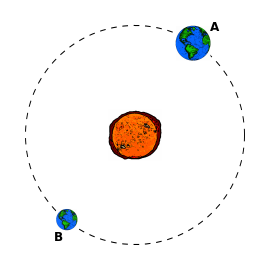
\includegraphics{../images/2PlanetsB.png}
	\end{center}
	
	\begin{TheSolution}
		A. Since the two are the same distance away from the star, the planet with the greater mass will experience the greater gravitational force from the star.
	\end{TheSolution}
	
	\part Planet $A$ is located \textbf{twice as far away} as planet $B$, but \textit{also} has \textbf{twice the mass} as planet $B$. Which, if any, experiences the greater gravitational attraction to the star? Why?
	\begin{center}
	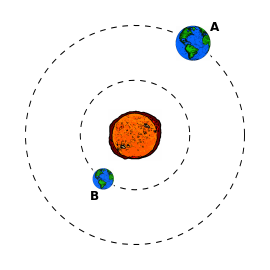
\includegraphics{../images/2PlanetsC.png}
	\end{center}
	\begin{TheSolution}
		B. The force of gravity is proportional to mass, but inversely proportional to the \textit{square} of the distance. Being 2 times as far means the force of gravity is 1/4 (not 1/2) the strength. Being 2 times the mass means the force is 2 times the strength. The net effect is that the force on planet $A$ is made smaller by a factor of 1/2 ($1/4 \cdot 2$).
		
		We can represent this with Newton's Law of gravitation. Let $M_S$ be the mass of the sun, and $m_B$ be the mass of planet $B$, $r_B$ be the distance for planet $B$, $m_A$ be the mass for planet $A$ and $r_A$ be the distance for planet $A$. The gravitational force experienced by planet $B$ is:
		\begin{eqnarray}
		F_B = G \frac{M_S m_B}{r_B^2} \nonumber
		\end{eqnarray}
		The gravitational force experienced by planet $A$ is:
		\begin{eqnarray}
			F_A = G\frac{M_s m_A}{r_A^2} = G\frac{M_s \times (2 m_B)}{(2 r_B)^2}  = G\frac{2M_S m_B}{4 r_B^2} = \frac{1}{2} G\frac{M_S m_B}{r_B^2}\nonumber
		\end{eqnarray}
		Which is 1/2 the force on planet $B$.
	\end{TheSolution}
	
	\end{parts}

\question The Earth's orbit around the Sun is not perfectly circular. Below is a (highly exaggerated) schematic of the Earth's elliptical orbit. Assume that energy is conserved in the Earth+Sun system.
\begin{center}
	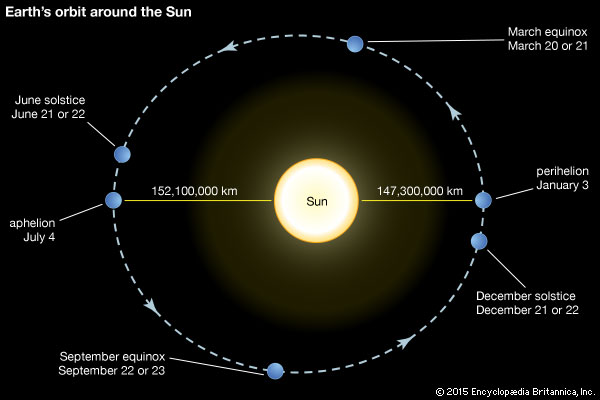
\includegraphics[width=0.7\textwidth]{../images/test2_seasons.jpg}
	\end{center}
	\begin{parts}
	\part When is the Earth moving the fastest around the Sun? When is it moving the slowest?
	\begin{TheSolution}
		The Earth is moving the fastest when its kinetic energy is the greatest. Since energy is conserved in this system, this happens when the potential energy is the least, when the Earth is closest to the Sun (at the perihelion, around January 3). The Earth is moving slowest when its kinetic energy is the least, when its potential energy is the greatest, when it is the farthest from the Sun, at the aphelion around July 4.
	\end{TheSolution}
	\part When does the Sun do positive work on the Earth? Negative work? Zero work?
	\begin{TheSolution}
	A force does positive work when it is pointing in the direction of the object's displacement. This occurs when the Earth is moving towards the Sun, from July 4 to January 3. The work is negative when the force from the Sun is opposite the direction of the Earth's displacement, when the Earth is moving away from the Sun, from January 3 to July 4. The work is zero when the force is perpendicular to the displacement, which happens at the exact moments the Earth is at the perihelion and aphelion.
	
	Another way of looking at this is that the Sun is doing positive work on the Earth when the Earth's kinetic energy is increasing and negative work when its kinetic energy is decreasing. The Earth's kinetic energy is decreasing as it moves towards the aphelion and increasing as it moves towards the perihelion.
		
	\end{TheSolution}
	\end{parts}

\question You are an astronaut looking for a new planet that reminds you of home.
\begin{parts}
\part You find a planet with three times the mass of Earth's and the same radius. How would the gravitational force on you on the surface of the planet compare to the gravitational force on you on the surface of the Earth?
\begin{TheSolution}
It would be three times stronger than on Earth.
\end{TheSolution}
\part You find a planet with the same mass as Earth and one half the radius. How would the gravitational force on you on the surface of the planet compare to the gravitational force on you on the surface of the Earth?
\begin{TheSolution}
It would be four times stronger than on Earth---you are at half the distance to the center of it.
\end{TheSolution}
\part You find a planet with four times the mass of Earth and twice the radius. How would the gravitational force on you on the surface of the planet compare to the gravitational force on you on the surface of the Earth?
\begin{TheSolution}
It would be the same as on Earth. The greater mass causes the force to be four times stronger, and the greater distance causes it to be four times weaker, so the two effects cancel out.
\end{TheSolution}
\end{parts}

\question Explain, using the properties of the electrostatic (Coulomb) force and the strong nuclear force, why all of the heaviest elements (elements with the most protons and neutrons in the nucleus) are unstable. Feel free to draw diagrams that help your explanation.
\begin{TheSolution}
This relates to the problem you did in class 5 to see why neutrons are necessary to keep a nucleus stable. The strong nuclear force only acts over very short range, so that nucleons (protons and neutrons) are only attracted to their nearest neighbours. Protons are repelled from other protons by the electrostatic force, so neutrons are required to increase the attractive binding energy of the nucleus and keep protons farther apart from each other (to screen them from their electrostatic repulsion). However, once there are too many protons in a nucleus, the amount that each proton is repelled by other protons is greater than the amount it is attracted to its nearest neighbours, and the nucleus is unstable and will eventually decay to produce two smaller nuclei. (There are quantum mechanical reasons you cannot make a nucleus with vastly more neutrons than protons in order to keep adding protons that are far enough apart that they aren't strongly repelled by each other.)
\end{TheSolution}

\question You are attempting to move a 20-kg cardboard box across a room and then upstairs. For each stage, describe the \textbf{change} in the box's energy, and say whether \textbf{you} did positive, negative, or zero work on the box. (For this problem, you can ignore the effects of air resistance but friction between the box and the floor is \textbf{not} negligible.)
\begin{center}
	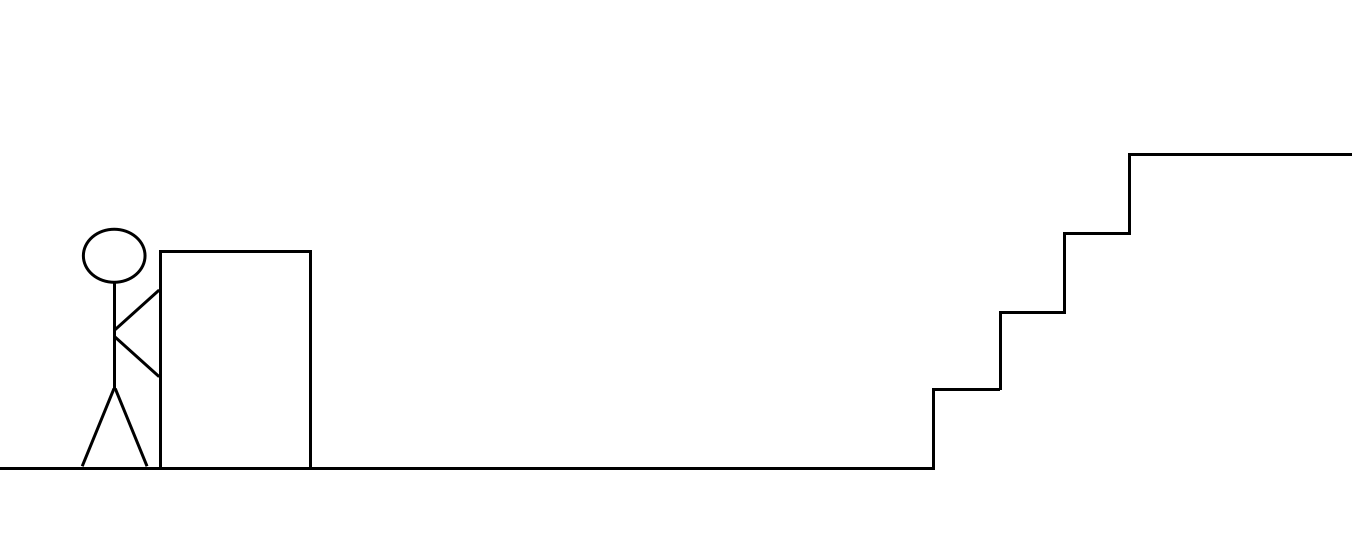
\includegraphics[width=0.7\textwidth]{../images/test2_stairs.png}
	\end{center}
\begin{parts}
\part You apply a horizontal force to the box as you accelerate from rest to 1 m/s in 1 s.
\begin{TheSolution}
The box's kinetic energy increases (by $\frac{1}{2}(20~\text{kg})(1~\text{m/s})^2 = 10~\text{J}$---it was not necessary for you to provide the exact amount though). You do positive work on the box.
\end{TheSolution}
\part You push the box at a constant velocity of 1 m/s for 5 s.
\begin{TheSolution}
The box's energy does not change. You do positive work on the box, to overcome friction.
\end{TheSolution}
\part You stop pushing the box and allow it to come to rest in 1 s.
\begin{TheSolution}
The box's kinetic energy decreases (by 10 J). You do no work on the box because you are not exerting a force on the box.
\end{TheSolution}
\part You lift the box to a height of 1 m.
\begin{TheSolution}
The box's potential energy increases (by $(20~\text{kg})(10~\text{m/s}^2)(1~\text{m}) = 200~\text{J}$). You do positive work on the box.
\end{TheSolution}
\part Holding the box at a constant height, you accelerate from rest to 1 m/s in 2 s.
\begin{TheSolution}
The box's kinetic energy increases (by $10~\text{J}$). You do positive work on the box.
\end{TheSolution}
\part You carry the box up a 3 meter flight of stairs at a constant speed of 1 m/s.
\begin{TheSolution}
The box's potential energy increases (by $(20~\text{kg})(10~\text{m/s}^2)(3~\text{m}) = 600~\text{J}$). You do positive work on the box.
\end{TheSolution}
\part You continue to carry the box at a constant height and a constant velocity of 1 m/s for 5 s.
\begin{TheSolution}
The box's energy does not change. You do no work on the box, since your force on the box is upwards and the box's displacement is forwards.
\end{TheSolution}
\part Holding the box at a constant height, you slow to a stop in 1 s.
\begin{TheSolution}
The box's kinetic energy decreases (by 10 J). You do negative work on the box.
\end{TheSolution}
\end{parts}

	
	\question
	What is the difference between \textbf{displacement} and \textbf{distance}? Describe a situation in which an object travels a nonzero distance, yet experiences zero displacement.
	\begin{TheSolution}
		Displacement describes the change in an object's position, regardless of the path it too. Distance is the total length of a path travelled by an object, regardless of direction.
		Situation: Walking down a hallway and coming back. The displacement is zero (since the final and initial position are the same) however the distance traveled would be twice the length of the hallway. (there are many other situations that would also work, as long as the final and initial position are the same).
	\end{TheSolution}
	
	\question
	What is the difference between \textbf{speed} and \textbf{velocity}? Describe a situation in which an object's speed is constant, but its velocity is changing.
	\begin{TheSolution}
		Speed describes an object's distance travelled per time, whereas a velocity describes an object's displacement per time and has a direction associated with it.
		Situation: Driving around a corner without accelerating or breaking. The speed is constant (the speedometer isn't changing) however the direction is changing, and thus velocity is changing. (there are many other situations that would also work).
	\end{TheSolution}	

	
	\question \textit{Particle accelerators}, as the name implies, are used to accelerate particles. These are used in a variety of experiments, such as colliders which smash particles together to better understand fundamental physics.
	
	Particles are not always accelerated at a constant rate, but rather experience ``acceleration bursts". The graph below shows the acceleration of a particle, as a function of time. There are 3 different ``acceleration bursts", (1) from 0~s~to~5~s, (2) from 6~s~to~11~s, and (3) 12~s~to~17~s.
	
	\begin{center}
	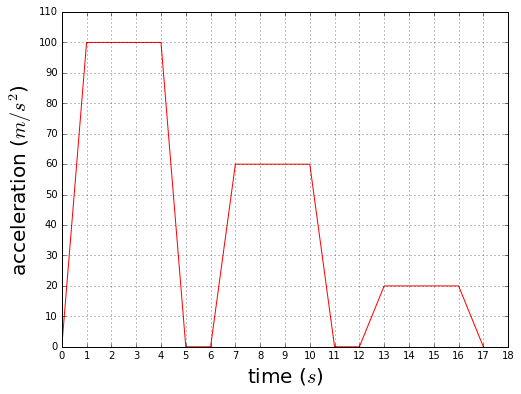
\includegraphics[width=4in]{../images/accelBursts.png}
	\end{center}
	
	\begin{parts}
		\part During which burst (1, 2 or 3) does the particle experience the \textbf{greatest change in velocity}? Please explain your answer.
			\begin{TheSolution}
				The area under an acceleration versus time graph is the change in velocity, and so the burst with the largest area will be the one that produces the greatest change in velocity. This is burst 1, from 0 to 5 seconds.
			\end{TheSolution}
			
		\part Describe the particle's motion from t=5~s to t=6~s.
			\begin{TheSolution}
				The object experiences no acceleration, and so must be moving at a constant velocity.
			\end{TheSolution}
		\part Assuming the particle begins at rest, when does the particle have the \textbf{greatest velocity}? What is this maximum velocity?
		\begin{TheSolution}
				The particle will have the greatest velocity at the point where there is the greatest area under the curve. This is at the end, from t=17~s onward. To calculate this velocity, we must calculate the total area under the graph. We do so for each burst, and add them all together:
				\begin{enumerate}
					\item $4~s \times 100~m/s^2 = 400~m/s$
					\item $4~s \times 60~m/s^2 = 240~m/s$
					\item $4~s \times 20~m/s^2 = 80~m/s$ 
				\end{enumerate}
				400~m/s + 240~m/s + 80~m/s = 720~m/s
			\end{TheSolution}
	\end{parts}

	\question
	Cars are designed with ``crumple zones", to reduce the impact of a collision on passengers. A person driving in winter skids on ice and collides their vehicle head on with a post. If they were initially traveling at 10~m/s, and during the crash the front compartment of their car crumples 1~m to absorb some of the impact, then:
	\begin{parts}
	\part What is the acceleration experienced by the driver in units of $m/s^2$? (\textbf{assume constant acceleration})
		\begin{TheSolution}
			We know the driver's initial velocity (10~m/s), final velocity (0~m/s) and the distance traveled (1~m). We are looking for the acceleration, and so we can use:
			\begin{eqnarray}
				v_f^2 &=& v_0^2 + 2 a \Delta x \nonumber \\
				(0~m/s)^2 &=& (10~m/s)^2 + 2 a\times(1~m) \nonumber \\
				0~m^2/s^2 &=& 100~m^s/s^s +  a\times(2~m) \nonumber 
			\end{eqnarray}
			We can rearrange the equation to solve for the acceleration, $a$:
			\begin{eqnarray}
				-100~m^2/s^2 &=&  a\times (2~m) \nonumber \\
				\Rightarrow a &=& \frac{-100~m^2/s^2}{2~m} = -50~m/s^2 \nonumber
			\end{eqnarray}
		\end{TheSolution}
	\part What is the acceleration experienced by the driver in units of $g = -10~m/s^2$?
		\begin{TheSolution}
			\begin{eqnarray}
			-50~m/s^2\times\frac{1~g}{-10~m/s^2} = 5~g \nonumber
			\end{eqnarray}
		\end{TheSolution}
	\part In order for the driver to experience an acceleration of $1.8~g$, what would their initial velocity need to be, assuming the car still crumpled by 1~m?
		\begin{TheSolution}
			Here, we have the acceleration (1.8~g), final velocity (0~m/s), distance traveled, and are looking for the initial velocity. We can reuse the same equation, only with different information. We first convert the acceleration fro $g$ to $m/s^2$:
			\begin{eqnarray}
			1.8~g\times \frac{-10~m/s^2}{1~g} = -18~m/s^2 \nonumber
			\end{eqnarray}
			And we can now use the same equation as before. We are now looking for $v_0$:
			\begin{eqnarray}
			v_f^2 &=& v_0^2 + 2 a \Delta x \nonumber \\
			(0~m/s)^2 &=& v_0^2 + 2(-18~m/s^2)(1~m)\nonumber \\
			0~m^2/s^2 &=& v_0^2 - 36~m^2/s^2 \nonumber
			\end{eqnarray}
			Rearranging the equation to solve for $v_0$, we get:
			\begin{eqnarray}
			36~m^2/s^2 &=& v_0^2 \nonumber \\
			\Rightarrow v_0 &=& \sqrt{36~m^2/s^2} = 6~m/s \nonumber
			\end{eqnarray}
		\end{TheSolution}
	\end{parts}
	
\question Two objects, each with mass $m$ and a positive charge $q$, are pushed towards each other with some velocity. The following 2 images show the two as they approach each other. Image $1$ represents their initial locations, where they are a distance $2r$ apart. Image $2$ shows their final positions, where they are a smaller distance $r$ apart. Use these images to answer the following questions.
\vspace{0.1in}
\begin{center}
\input{../images/2massCharges.pdf_tex}
\end{center}
\vspace{0.1in}
\begin{parts}
	\part Is it possible to tell how the electric force between them changes? If so, does it increase, decrease or stay the same?
		\begin{TheSolution}
			Increase. The electric force increases as the two are brought closer together. The charges are repelling each other, and repel each other more as they are forced closer together.
		\end{TheSolution}
	\part Is it possible to tell how the electric potential energy changes? If so, does it increase, decrease or stay the same?
		\begin{TheSolution}
			Increase. The electric potential energy increases as they are brought closer together.
		\end{TheSolution}
	\part Is it possible to tell how the gravitational force between them changes? If so, does it increase, decrease or stay the same?
		\begin{TheSolution}
			Increase. The gravitational force between them increases, since they are closer together. The gravitational force is attractive, and the closer they are the more they attract each other.
		\end{TheSolution}
	\part Is it possible to tell how the gravitational potential energy changes? If so, does it increase, decrease or stay the same?
		\begin{TheSolution}
			Decrease. The gravitational potential energy decreases, since gravity is an attractive force.
		\end{TheSolution}
\end{parts}

\end{questions}

\end{document}
